	\thispagestyle{empty}
	
	\begin {center}
	\begin{tabular} {|p {3cm}|p{8cm}|p{4.55cm}|}
	 \hline 
	\vspace{1mm}
	 \centering{
\includegraphics[width=0.20\textwidth,page=1]{Alle/TGM_logo.pdf}} &
	\centering{\normalsize{\textbf{HTBLVA Wien 20}}\par\small{\textbf{College of}\par Biomedical Engineering}} &
		\small{\bfseries{Diploma\par Exam}}\\ 
		\hline
	\end{tabular}
	
	\vspace{5mm}
	\Large{\textbf{DIPLOMA THESIS\\}}
	\vspace{1mm}
	\small{\textbf{DOCUMENTATION\\}}
	\vspace{5mm}  
	
		\begin{tabular} {|p {5.7cm}|p{10.3cm}|}
		 \hline 
			\bfseries{\small{Authors}} & \small{Fatiha Banata, Claudia Fuchs, Julia Gartner, Sumaiya Hossain}\\
		 \hline
		  \bfseries{\small{From\par Academic year}} & \small{5AHBG 2022/2023}\\
		 \hline 
		  \bfseries{\small{Topic}} & \small{Sleep-Analyzer}\\ 
		 \hline 
		  \bfseries{\small{CO-operation partners}} & \small{/}\\ 
		 \hline
		\multicolumn{2}{l}{\large{ \textbf{}}}\\
		 \hline
		  \bfseries{\small{Assignment of tasks}} & \small{A prototype to analyze sleep has to be developed. This prototype should be able to measure appropriate biosignals of an sleeping user. The goal is to test and evaluate the functionaltity of such a prototype.}\\
		 \hline
		\multicolumn{2}{l}{\large{ \textbf{}}}\\ 
		 \hline
		  \bfseries{\small{Realization}} & \small{In order to detect the REM-sleeping phase, an Electorokulogram that detects eye movements has been developed. The data is measured by an ESP8862 and sent to a database via wifi. The user is able to get feedback of the data in an app interface.}\\  
		 \hline
		\multicolumn{2}{l}{\large{ \textbf{}}}\\ 
		 \hline
		  \bfseries{\small{Results}} & \small{Eye movements can be detected and be timestamped with an RTC-module. The ESP-database connection works. }\\
		 \hline 
		\end{tabular}
	\end {center}
	
\thispagestyle{empty}
		
\newpage
\thispagestyle{empty}

	\begin{centering}
	\begin{tabular} {|p {3cm}|p{8cm}|p{4.55cm}|}
	 \hline 
	\vspace{1mm}
	 \centering{
\includegraphics[width=0.20\textwidth,page=1]{Alle/TGM_logo.pdf}} &
	\centering{\normalsize{\textbf{HTBLVA Wien 20}}\par\small{\textbf{College of}\par Biomedical Engineering}} &
		\small{\bfseries{Diploma\par Exam}}\\ 
		\hline
	\end{tabular}
	
   \vspace {2mm}
	
		\begin{tabular} {|p {5.7cm}|p{10.3cm}|}
		 \hline 
			\bfseries{\small{Illustrative graph, photo\par (with explanation)}} & \vspace{0.0mm} \small{
			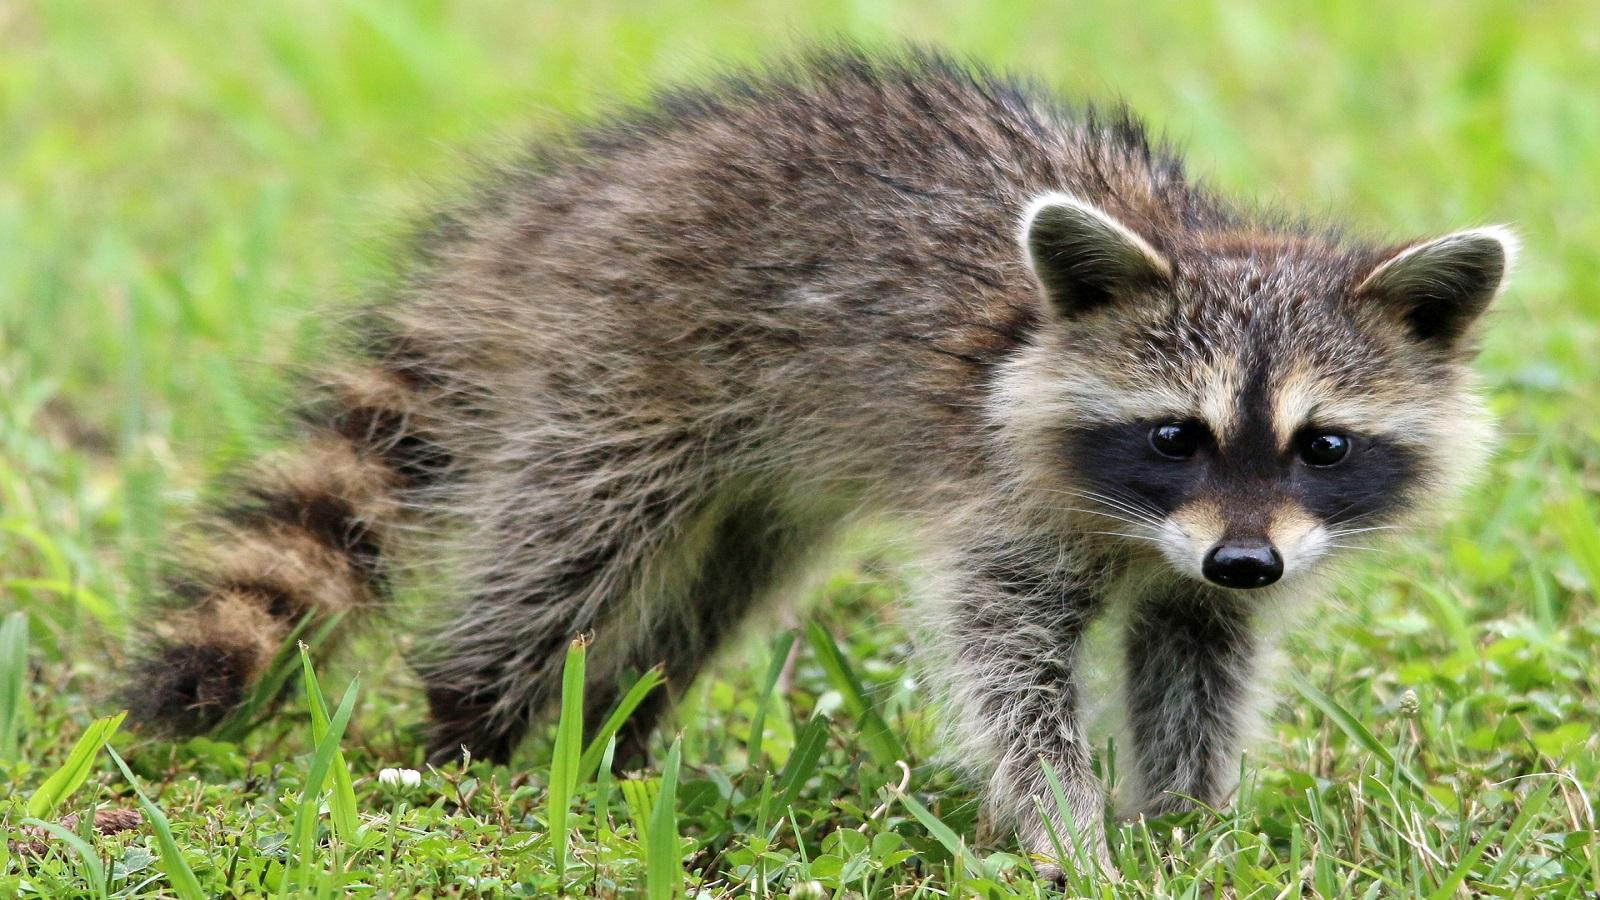
\includegraphics[width=0.666\textwidth]{Alle/Bild.jpg} \par BILDBESCHREIBUNG
			}\\
		 \hline
		  \multicolumn{2}{l}{\large{ \textbf{}}}\\
		 \hline
		  \bfseries{\small{Participation in competitions,\par Awards}} & \small{/}\\
		 \hline 
		  \multicolumn{2}{l}{\large{ \textbf{}}}\\
		 \hline
		  \bfseries{\small{Accesibility
			of\par Diploma Thesis}} & \small{Department administration}\\ 
		 \hline 
		  \multicolumn{2}{l}{\large{ \textbf{}}}\\
		\end{tabular}  
		
		\begin{tabular} {|p {5.7cm}|p{5.3cm}|p{4.6cm}|}
		 \hline
	   \vspace{5mm}
		  \bfseries{\small{Approval\par (Date/Signature)}} \vspace{5mm} & \tiny{Examiner} & \tiny{Head of College/Department}\\ 
		 \hline 
		\end{tabular} 
		\end{centering}

\thispagestyle{empty}
